\section{大气压的变化 气压计}\label{sec:5-12}

在托里拆利用实验测出了大气压的值以后,帕斯卡想到,既然大气压是由大气层受到的重力产生的,
那么,离地面越高,大气层的厚度越薄,那里的大气压应该越小。因此,山顶上的大气压应该比山脚下的大气压小。
为了证实这个想法,帕斯卡和他的朋友于 1648 年同时在山顶和山脚下做了托里拆利实验。实验结果完全证实了帕斯卡的想法。

离地面越高,空气越稀薄,空气的密度越小。因此,大气压随高度而减小是不均匀的,越高大气压随高度减小得越慢。
在海拔 2 千米以内,可以近似地认为每升高 12 米,大气压降低 133 帕斯卡,即约 1 毫米汞柱。
利用这个近似的规律,测出某处大气压的值,就可以计算出那个地方的大致高度。

托里拆利在多次做他的著名实验的时候,还观察到在不同时间,在同一地方大气压的值并不完全相同。
研究表明,大气压的变化跟天气有密切的关系。一般地说,晴天的大气压比阴天的高,冬天的大气压比夏天的高。
因此,测量大气压就成为天气预报的重要依据之一。

由于大气压的值不是固定不变的,通常把等于 760 毫米汞柱的大气压叫做\textbf{标准大气压}。

气象台站要经常测量大气压,用来测量大气压的仪器叫做\textbf{气压计}。
在托里拆利实验中,如果在装水银的玻璃管旁固定一个刻度尺,就可以直接读出大气压的值,
这就做成了一个气压计,这种气压计叫做水银气压计。

\begin{figure}[htbp]
    \centering
    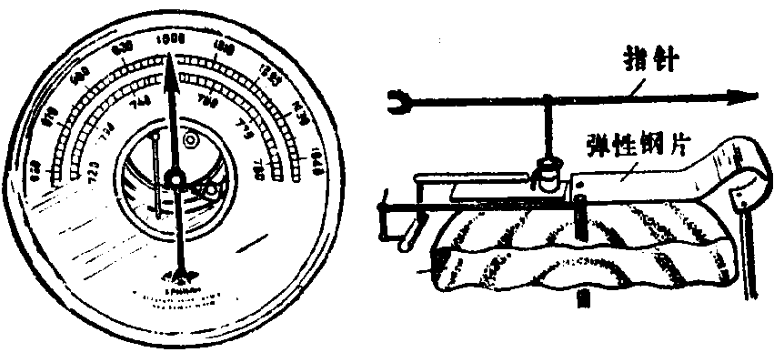
\includegraphics[width=0.7\textwidth]{../pic/czwl1-ch5-45}
    \caption{无液气压计}\label{fig:5-45}
\end{figure}

水银气压计测量结果准确,但是携带不方便。实际上常用的气压计是金属盒气压计,也叫无液气压计。
它的构造如图 \ref{fig:5-45} 所示,主要部分是一个表面为波纹状的金属盒,盒内的空气已经抽出。
为了使金属盒不被大气压压扁,金属盒盖用弹性钢片向外拉着。
大气压增大时,盒盖就凹进去一些,大气压减小时,弹性钢片就把盒盖拉出来一些。
盒盖的变化传给指针,从指针指示的刻度,就可以读出大气压的值。

如果无液气压计的刻度盘上标的不是大气压的值,而是高度,就成了航空、登山用的高度计。

